\documentclass[twoside]{article} \usepackage{aistats2017}

% If your paper is accepted, change the options for the package
% aistats2017 as follows:
%
%\usepackage[accepted]{aistats2017}
%
% This option will print headings for the title of your paper and
% headings for the authors names, plus a copyright note at the end of
% the first column of the first page.
\usepackage{color}
\usepackage{natbib}
\usepackage{url}
\usepackage{amsmath}
\usepackage{amsfonts}
\usepackage{stackengine}
\usepackage{graphicx}
\usepackage{subcaption}

\usepackage[colorlinks]{hyperref}
\usepackage{cleveref}


\renewcommand{\deg}{\ensuremath{^\circ}}
\newcommand{\cov}{\text{cov}}
\newcommand{\N}{\mathcal{N}}
\renewcommand{\v}[1]{\mathbf{#1}}
\newcommand{\ve}{\v{\varepsilon}}
\newcommand{\todo}[1]{{\color{red} \textbf{TODO:} {#1}}}

\begin{document}

% If your paper is accepted and the title of your paper is very long,
% the style will print as headings an error message. Use the following
% command to supply a shorter title of your paper so that it can be
% used as headings.
%
%\runningtitle{I use this title instead because the last one was very long}

% If your paper is accepted and the number of authors is large, the
% style will print as headings an error message. Use the following
% command to supply a shorter version of the authors names so that
% they can be used as headings (for example, use only the surnames)
%
%\runningauthor{Surname 1, Surname 2, Surname 3, ...., Surname n}

\twocolumn[

\aistatstitle{Signal-based Bayesian Seismic Monitoring}

\aistatsauthor{ Dave Moore \And Stuart Russell}

\aistatsaddress{ University of California, Berkeley } ]

\begin{abstract}
  We present a Bayesian generative model of seismic events and signals
  observed across a network of spatially distributed sensors. Our
  system directly models seismic waveforms, incorporating a rich
  representation of the physics underlying the signal generation
  process. We use Gaussian processes to predict detailed waveform
  fluctuations based on historical events, while degrading smoothly to
  simple parametric envelopes in regions with no historical
  seismicity. Our system combines the qualitative advantages of
  existing monitoring approaches that use bottom-up detections and
  waveform matching, in a unified Bayesian model with principled
  treatment of uncertainty. Evaluating on data from the western
  US, we recover three times as many events as previous work,
  and reduce mean location errors by a factor of four while greatly increasing
sensitivity to low-magnitude events. 
\end{abstract}

\section{Introduction}

The world contains structure: objects, forces, and dynamics governed by
physical law. Intelligent systems must learn to infer this structure
from noisy, jumbled, and lossy sensory data. Bayesian statistics
provides a natural framework for designing such systems: given a prior distribution
$p(z)$ on underlying descriptions of the world, and a forward model $p(x|z)$
describing the process by which observations are generated,
mathematical probability defines the posterior $p(z|x) \propto p(z)p(x|z)$ over worlds
given observed data. 

This paper applies the Bayesian framework directly to a
challenging perceptual task: monitoring seismic events from a network
of spatially distributed sensors. In addition to obvious applications
to seismology, this task is motivated by the Comprehensive Test Ban
Treaty (CTBT), which bans testing of nuclear weapons and provides for
the establishment of an International Monitoring System (IMS) to
detect potential treaty violations. Because underground nuclear tests
register as low-magnitude seismic events, the ability to detect such
events from noisy data at distant sensors is critical to the success of the
treaty. The inadequacy of existing monitoring systems was cited as a
factor in the US Senate's 1999 decision not to ratify the treaty. 

Our system, SIGVISA (Signal-based Vertically Integrated Seismic
Analysis), consists of a generative probability model of seismic
events and signals, with interpretable latent variables corresponding
to physically meaningful quantities such as the arrival times and
amplitudes of seismic phases. By incorporating physics-based
predictive models in tandem with Gaussian processes learned from
historical data, our forward model produces reasonable predictions
even in regions with no nearby training events. Bayesian inference in
this model recovers a posterior over event bulletins directly from
seismic waveforms, combining top-down with bottom-up processing to
produce a joint interpretation of all observed data, while avoiding
preprocessing steps that discard information. 

We begin with a brief primer on the physics
underlying seismic signal generation. We then describe the SIGVISA generative
model, including a collapsed form that is more amenable to efficient
inference, and outline MCMC and EM-based procedures for inference and
training, respectively. We finally evaluate the event bulletins
produced by our system through a comparison to existing monitoring
systems on two weeks of data from the western United States, for which
a regional reference bulletin is available to serve as approximate
ground truth. We find that SIGVISA recovers substantially more events
than existing systems, reducing detection thresholds by up to an
order of magnitude and location error by a factor of four, while
performing as well or better than existing systems on events with no
nearby historical seismicity. 

\todo{Due to space limits it is not possible to describe every aspect
  of our model and inference procedures in this short paper. We
  attempt to illustrate the key points but will occasionally defer to 
  \citep{thesis} for additional details. }

%This allows us to
%define a rich forward model incorporating the local waveform
%similarities exploited by correlation detectors, along with the phase
%travel time and attenuation structure used by detection-based systems,
%in a single unified model. Inference in this model recovers the
%qualitative advantages of both approaches, incorporating evidence from
%each according to their uncertainties.

\section{Seismic Background}

\begin{figure}
\centering
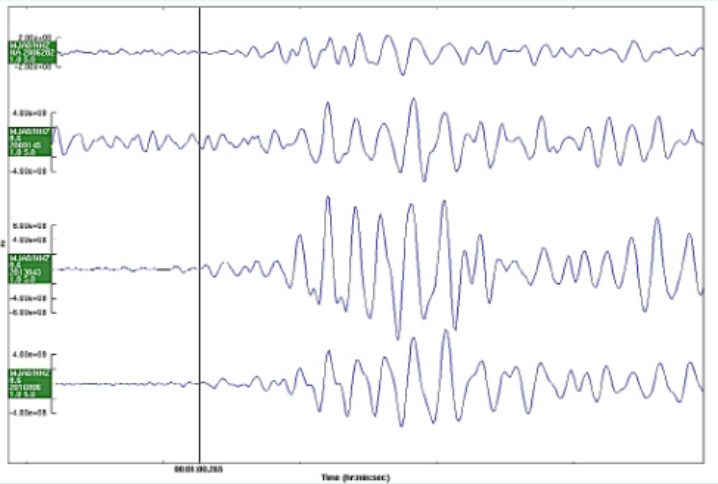
\includegraphics[width=0.45\textwidth]{correlation_dprk}
\caption{\todo{replace with overlayed figure}}
\label{fig:dprk_correlations}
\end{figure}

We model seismic events as point sources, localized in space and time,
that release energy in the form of seismic waves. These include
compression waves (``P waves'') and shear waves (``S waves'') that
travel through the solid earth, as well as {\em surface} waves such as
Love and Rayleigh waves, which propagate along the surface and are
responsible for most earthquake damage. Waves are further categorized
into {\em phases}, e.g., Pg, Pb, Pn, etc., according to the paths they traverse from a source to a detecting station. 

Given an event's location, it is possible to predict the arrival time of each phase by
considering the length and characteristics of the event--station
path; by inverting these predictions we can locate events given
a set of phase arrival times.  Seismologists have developed a number of phase travel
time models, ranging from simple models that condition only on event
depth and event-station distance \citep{iaspei91}, to more sophisticated models
that use an event's precise location to provide more
accurate predictions incorporating the local velocity structure \citep{simmons2012llnl}. Our system
treats the travel-time model as a black box, allowing us to easily incorporate improvements from domain experts. 

Seismic stations record continuous ground motion along one or more
axes,\footnote{In this work we consider vertical motion only.} including background noise from natural and human sources, as well as the
signals generated by arriving phases of seismic events. The detailed
fluctuations in these signals are a function of the source  as well as a path-dependent transfer function,
in which seismic energy is modulated and distorted by the geological
characteristics of the paths followed by each phase. Since
event--station paths are themselves functions of the source location,
events with similar locations and depths tend to generate
highly correlated waveforms as long as the source mechanisms are not
too different (\Cref{fig:dprk_correlations}). The lengthscale at which such
correlations are observed depends on the local geology and may range
from hundreds of meters up to tens of kilometers. Since wave propagation is
essentially deterministic and geological structures are essentially static
on human timescales, significant correlations can be observed even
from events occurring decades apart. 

\todo{reference figure with envelope model of real signals?}

\subsection{Monitoring systems}

\begin{figure}
\centering
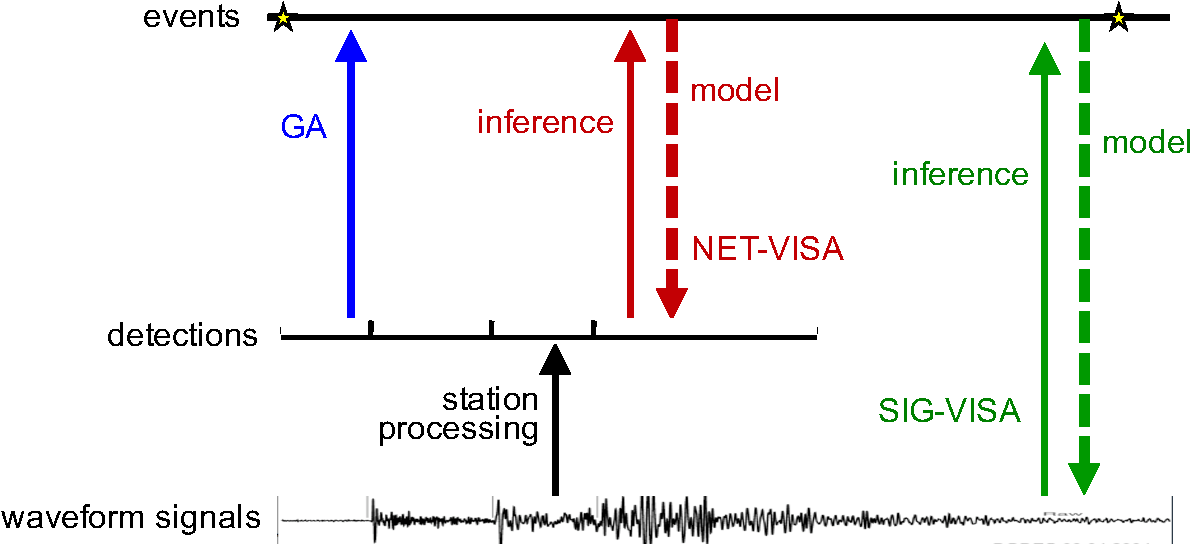
\includegraphics[width=.45\textwidth]{netvisa_sigvisa-crop}
\caption{High level structure of traditional monitoring (GA), detection-based Bayesian monitoring (NETVISA), and signal-based Bayesian monitoring (SIGVISA, this work). Where GA and NETVISA are limited to detections produced by bottom-up station processing, inference in a signal-based model incorporates much richer information from the signals themselves.}
\label{fig:monitoring_comparison}
\end{figure}

Traditional approaches to seismic monitoring proceed via bottom-up
processing. The waveform at each station is thresholded to
produce a feature representation consisting of discrete ``detections'' of possible phase
arrivals. {\em
  Network processing} attempts to associate detections from
all stations into a coherent set of events. In addition to the
inherent combinatorial task, network processing is complicated by
false detections, caused by noise, and missing detections, from
arrivals for which the station processing failed to trigger.
In addition, the limited information provided by a single detection
(estimates of arrival time, amplitude, and in some cases
directional information) means that at least three
separate stations are typically required for reliable event
formation. 

The NETVISA system \citep{arora2010global,arora2013net} replaces heuristic network
processing with inference in a principled Bayesian model of seismic
events and detections, including models of false and missing
detections. Maximizing posterior probability in this model via
hill-climbing search yields an event bulletin based on all available
data, accounting for uncertainty, and additionally separates
the construction of an explicit domain model from the design of
inference algorithms, so that the system can be interpreted and
improved by domain experts. Results include significant improvements
in location accuracy and a 60\% reduction in missed events compared to
the SEL3 bulletin produced by the previous network processing system (Glocal
Association, or GA) in use by the IMS \citep{arora2013net}. As of this
writing, NETVISA has been proposed as the new production monitoring
system for the CTBT, pending approval by the member states. 

Recently, new monitoring approaches have been proposed using the
principle of {\em waveform matching}, which exploits correlations
between signals from nearby events to detect and
locate new events by matching incoming signals against a library of
historical signals. These promise the ability
to detect events up to an order of magnitude below the threshold of a
detection-based system \citep{gibbons2006detection,schaff2010one}, and
to locate such events even from a single station, greatly increasing
the sensitivity of monitoring networks
\citep{schaff2012seismological}. However, adoption has been hampered by their inability to detect
events in locations with no historical seismicity, a crucial requirement
for nuclear monitoring. In addition, it has not been clear how to quantify
the uncertainty in events detected by waveform correlation, how to
combine potentially conflicting correlations from different stations,
or how to bridge the divide between correlation and detection-based
methods. 

\section{Model}

\begin{figure}
\centering
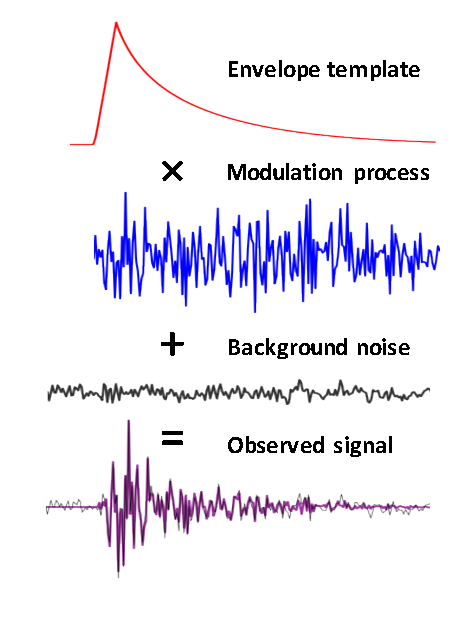
\includegraphics[width=.35\textwidth]{model_algebra_cropped}
\caption{Forward model for a single phase arrival.}
\label{fig:model_algebra}
\end{figure}

The current work, SIGVISA, extends NETVISA by eliminating bottom-up
detection processing in favor of joint inference in a principled
Bayesian model of seismic events and signals. Our model describes a joint distribution
$p(\v{E}, \v{S}) = p(\v{S}|\v{E})p(\v{E})$ on seismic events $\v{E}$ and 
signals $\v{S}$ observed across a network of $n_S$ stations. We model event occurrence as a time-homogenous Poisson process,
\begin{align*}
p(n_E) &= \text{Poisson}(\lambda T)\\
p(\v{E}) &= p(n_E) n_E! \prod_{i=1}^{n_E} p(\v{e}_i)
\end{align*}
so that the number of events $n_E$ generated during a time period of
length $T$ is itself random, and each event is sampled independently from
a prior $p(\v{e}_i)$ over surface location, depth, origin time, and
magnitude. Note the Poisson process induces a uniform prior on origin
times, with a labeling symmetry that we correct by multiplying by the
permutation count $n_E!$. The remaining priors, along with the event
rate $\lambda$, are estimated from historical seismicity as described in \citep{netvisa}. In
particular, the location prior is a mixture of a kernel density
estimate of historical events, and a uniform component to allow events
(such as explosions) in locations with no previous seismicity.

We assume that signals at different stations are
conditionally independent, given events, and introduce auxiliary
variables $(\v{\theta}, \v{w})$ governing signal generation at each
station, so that the forward model has the form
\begin{equation}
p(\v{S}|\v{E}) = \prod_{j=1}^{n_S} \int p(\v{s}_j | \v{\theta}_j, \v{w}_j)p(\v{\theta}_j|\v{E}) p(\v{w}_j| \v{E}) d\v{w} d\v{\theta}.
\end{equation}
The variables $\v{\theta}$ and $\v{w}$ describe, respectively, the
signal envelope generated by arriving phases, and a modulation process
that multiplies the envelope to generate the observed waveforms. In
particular, they decompose into independent $\v{\theta}_{i,j,k}$ and
$\v{w}_{i,j,k}$ describing the arrival of phase $k$ of event $i$ at
station $j$. The set of phases generated by a particular event is
taken to be a near-deterministic function of depth and event--station distance.

We model the envelope generated by each phase
arrival as a linear onset followed by a poly-exponential decay, 
\begin{equation}g(t; \theta_{i,j,k}) = \left\{\begin{array}{ll}
0 & \text{ if } t \le \tau\\
\alpha (t-\tau) / \rho & \text{ if } \tau < t \le \tau+\rho\\
\alpha (t-\tau+1)^{-\gamma} e^{-\beta (t-\tau)} &\text{ otherwise}\\
\end{array}\right.\end{equation}
parameterized by $\theta_{i,j,k} = (\tau, \rho, \alpha, \gamma,
\beta)_{i,j,k}$ consisting of an arrival time $\tau$, rise time $\rho$, amplitude
$\alpha$, and decay rates $\gamma$ and $\beta$ governing respectively
the envelope peak and its long-run coda. This decay form is inspired by previous work modeling seismic
coda \citep{mayeda2003stable}, while the linear
onset follows that used by 
\citet{cua2005creating} for seismic early warning. \Cref{fig:envelopes} illustrates the envelope
form $g$ with examples fit to real seismic phase arrivals.

The signal generated by a phase arrival is modeled
as the envelope times a {\em modulation process} $m$, parameterized
by wavelet coefficients $\v{w}_{i,j,k}$ so that
\begin{equation}
m(t; \v{w}_{i,j,k}) = \left\{\begin{array}{ll} (\mathbf{D}\v{w}_{i,j,k})(t) & \text{if } 0 \le t <
                                                    20s\\\ve(t) & \text{otherwise}\end{array}\right.\end{equation}
where $\mathbf{D}$ is a discrete wavelet transform, and
$\ve(t)\sim\N(0, 1)$ is a Gaussian white noise process. We
explicity represent wavelet coefficients describing the first 20
seconds\footnote{This cutoff was chosen to
  capture repeatability of the initial arrival period, which is
  typically the most clearly observed, while still fitting historical
  models in memory.} of modulation for each 
phase, and model it as random after that point. We use an order-4 Daubechies wavelet
basis \citep{daubechies1992ten}, so that for 10Hz signals each
$\v{w}_{i,j,k}$ is a vector of 220 coefficients.  As described below, we
model $\v{w}$ jointly across events using a Gaussian process, so that
our modulation processes are {\em repeatable}: events in nearby locations
will generate correlated signals. 

Given the envelope shapes and modulation processes, we sum over all
arriving phases at station $j$ to construct a {\em predicted signal} $\v{\bar{s}}_j$,
\begin{equation}
\bar{s}_j(t) = \sum_{i, k} g(t; \v{\theta}_{i,j,k})\cdot m(t-\tau_{i,j,k}; \v{w}_{i,j,k}).
\end{equation}
The observed signal $\v{s_j}$ incorporates background noise from an
order-$R$ autoregressive process,
\begin{align}
p(\v{s}_j | \v{\theta}_j, \v{w}_j) = p_{AR}(\v{s}_j - \v{\bar{s}}_j - \mu_j;
\sigma^2_j, \v{\phi}_j)\\
p_{AR}(\v{s}; \sigma^2, \v{\phi}) = \prod_{t=1}^T \N\left(s(t);
\sum_{r=1}^R \v{\phi}_r s(t-r), \sigma^2_r\right)\nonumber
\end{align}
where $\mu_j$, $\sigma^2_j$, and $\v{\phi}_j$ are station-specific
parameters governing the noise mean, variance, and autoregressive
dependence, respectively. \Cref{fig:signals} illustrates our model of
signal generation. 

\subsection{Repeatable signal descriptions}

We model the signal
descriptions $\v{\theta}_{j,k}$ and $\v{w}_{j,k}$, for each station
$j$ and phase $k$, jointly as Gaussian process \citep{rasmussen2006}
transformations of the event space $\v{E}$, so that events in
nearby locations will tend to generate similar envelope shapes, up to
magnitude scaling, and correlated modulation signals, allowing our system to
detect and locate repeated events even from a weak signal recorded at a single
station. Since the input (event) locations are unknown, this is effectively a
GP latent variable model \citep{gplvm}, although in our model the
the outputs $\v{\theta}, \v{w}$ are themselves latent
variables that we observe only indirectly through the noisy signals $\v{S}$. The flexibility
of a GP modeling framework allows us to combine physics-derived mean
predictions, learned parametric components that generalize to novel event
locations (e.g., modeling amplitude as a function of event-station
distance), and nonparametric components with the capacity to exactly
match historical signals. 

We borrow models from geophysics to predict the arrival time and
amplitude of each phase. Given the origin time, depth, and
event-station distance, the IASPEI-91 \citep{iaspei91} travel-time
model predicts an arrival time $\bar{\tau}$, and the Brune
source model \citep{brune} predicts a source (log) amplitude
$\log \bar{\alpha}$ as a function of event magnitude. We then use
GPs to model deviations from these physics-based predictions; that is,
we take $\bar{\tau}$ and $\log \bar{\alpha}$ as the
mean functions for GPs modeling $\tau$ and $\log
\alpha$ respectively. The remaining shape parameters $\rho, \gamma,
\beta$ (in log space) and the 220 wavelet coefficients in $\v{w}_{i,j,k}$ are also
modeled by independent zero-mean GPs. 

\begin{table}
\centering
\begin{tabular}{ll}
\hline
\textbf{Parameter} & \textbf{Features $\phi(\v{e})$} \\\hline
Arrival time ($\tau$) & n/a  \\
Amplitude (log $\alpha$) & $\left(1,\delta,\sin(\frac{\delta}{15000}),
                           \cos(\frac{\delta}{15000})\right)$ \\
Onset (log $\rho$) & (1, mb) \\
Peak decay (log $\gamma$) & (1, mb, $\delta$) \\
Coda decay (log $\beta$) & (1, mb, $\delta$) \\
Wavelet coefs ($w$) & n/a \\\hline
\end{tabular}
\caption{Feature representations in terms
  of magnitude mb and event--station distance $\delta$ (km).}
\label{tbl:gp_models}
\end{table}

All of our GPs share a common covariance form,
\[k(\v{e}, \v{e}') = \phi(\v{e})^T \v{B}\phi(\v{e}') + \sigma^2_f
k_\text{Mat\'ern}(d_\ell(\v{e}, \v{e}')) + \sigma^2_n \delta(\v{e},
\v{e}').\]
The first term models an unknown function that is linear in some
feature representation $\phi$ (\Cref{tbl:gp_models}), with prior
weight covariance $\v{B}$. For efficiency and to avoid degenerate
covariances we represent this component in weight space, as discussed
by \citet[section 2.7]{rasmussen2006}; at test time we choose $\v{B}$
to be the posterior weight covariance from conditioning on training
data under a noninformative prior. The second term models an unknown
differentiable function using a stationary Mat\'ern ($\nu=3/2$) covariance \citep[Chapter
4]{rasmussen2006}, with great-circle distance metric controlled by
lengthscale hyperparameters $\ell$. This allows our model to represent
detailed local seismic structure, while the linear term enables
generalization to novel locations. We also include an i.i.d. Gaussian noise
term $\sigma^2_n \delta(\v{e}, \v{e}')$ to encode unmodeled factors that may cause signals to vary
between events in the same location.

To enable efficient training and test-time predictions from GP models,
we partition the training data using $k$-means clustering into spatially local regions, and impose
independence across regions on the nonparametric Mat\'ern
component. This allows predictions in each region to be made efficiently
using only a small number of nearby events, avoiding the na\"ive
$O(n^2)$ dependence on the entire training set. We also learn separate
hyperparameters for each region, so that the local factorization allows
our models to adapt to spatially local regions.
\todo{include a picture of factored GP?}

%We do not
%factorize the parametric component $\phi(\v{e})^T \v{B}\phi(\v{e}')$,
%which models global structure and is already independent of the
%training set size due to the weight-space representation. 

\subsection{Collapsed signal model}

The explicit model described thus far exhibits tight coupling between
envelope parameters and modulation coefficients; a small shift in a
phase's arrival time may significantly change the wavelets needed to
explain an observed signal. Fortunately, it is possible to exactly
marginalize out the coefficients $\v{w}$ so that they do not need to
be represented in inference. This follows from the linear Gaussian
structure of our signal model: GPs induce a Gaussian distribution on
wavelet coefficients, which are observed under linear projection (a
wavelet transform followed by envelope scaling) with autoregressive
background noise. Thus, the collapsed distribution
$p(\v{s}_j | \v{\theta}_j, \v{E}) = \int p(\v{s}_j | \v{\theta}_j, \v{w}_j)
p(\v{w}_j | \v{E}) d\v{w}_j$
is multivariate Gaussian, and in principle we can evaluate this density
directly without reference to an explicit wavelet representation.

In practice, to do this efficiently we must exploit graphical model
structure. Specifically, we formulate the signal model at each station 
as a linear Gaussian state space model, with a state vector
that tracks the autoregressive noise process as well as the set of
wavelet coefficients that actively contribute to the signal at each
timestep.  Due to the recursive structure of wavelet bases, the number
of active coefficients at a given time is logarithmic in the size of
the basis; this is exploited by fast wavelet transforms. In a
probabilistic setting the same structure allows us to efficiently\footnote{Requiring time linear in the signal length; more precisely,
  $O(T (K \log C + R)^2 )$ for a signal of length $T$ with order-$R$
  AR noise and at most $K$ simultaneous phase arrivals, each described
  by $C$ wavelet coefficients.} compute coefficient posteriors and
marginal likelihoods by Kalman filtering
\citep{kalmanref}. 

For efficiency at test time we assume that signals from different
events are independent given the training data. However, to
infer correct alignments during training it is necessary to compute
the joint density of signals involving multiple events, requiring us to
pass messages from each event upwards to the GP prior
\citep{koller2009probabilistic}. We approximate the true messages $f_j(\v{w}_j) =
p(\v{s}_j | \v{w}_j, \v{\theta}_j)$ with diagonal
messages \[\tilde{f}_j(\v{w}_j) = \frac{1}{Z_j}\prod_{c=1}^{220} \N(\v{w}_{j,c};
\tilde{\nu}_{j,c}, \tilde{\xi}_{j,c})\] computed by dividing the Kalman
filtering posterior on wavelet coefficients by the (diagonal Gaussian)
prior. The product of these messages with the GP prior $p(\v{w}_c | \v{E})
\sim \N(\v{\mu}_c(\v{E}), \v{K}_c(\v{E}) )$, integrated over coefficients $\v{w}$, gives an approximate
joint density
\begin{equation}
p(\v{S} | \v{E}, \v{\theta}) \approx \left(\prod_{j=1}^N
  \frac{1}{Z_j} \right) \prod_c \N\left(\bar{\nu}_c; \v{\mu}_c(\v{E}),   \v{K}_c(\v{E}) + \v{\xi}_{c} \right)\label{eqn:efficient_joint_density},
\end{equation}
in which the wavelet GPs are evaluated at the values of (and
with added variance given by) the messages. We target this
approximate joint density during training, and condition our test-time
models on the upwards messages generated by training signals. 

\section{Inference}

We perform inference using reversible jump MCMC \citep{rjmcmc} applied
to the collapsed model. Our algorithm consists of a cyclic sweep of
single-site random-walk Metropolis-Hastings (MH) proposals over all currently
instantiated envelope parameters $\v{\theta}$, autoregressive noise
parameters $\mu, \sigma^2, \phi$ at each station, and event
descriptions $(\v{e}_i)_{i=1}^{n_E}$ including surface location,
depth, time, and magnitude. We also include custom
moves that propose swapping the associations of consecutive arrivals, shifting arrival times to
increase the correlation between the predicted and observed signal,
and shifting phase envelope peaks to match peaks in the envelope of
the observed signal. 

To enhance event mixing, we augment our model to allow {\em unassociated
  arrivals}: phase arrivals not generated by any particular event, with a fixed Gaussian prior on envelope parameters and modulation signals. These are useful in allowing events to be built
(and destroyed) piecewise, as opposed to requiring us to perfectly
propose an event and all its phases in a single shot. They can also be
thought of individually as small events whose locations have been
(roughly speaking) integrated out, since some events detected only
at a single station cannot be localized. Our birth
proposal generates arrivals with probability proportional
to the signal envelope, so that periods of high signal energy are
quickly explained by unassociated arrivals, which may then be
associated into larger events.\footnote{In this sense the unassociated
arrivals play a role similar to the detections produced by traditional
station processing. However, they are not generated by bottom-up
preprocessing, but as part of a dynamic inference procedure that may
create or destroy them based on observed signals as well as top-down
event hypotheses.}

We define two separate event birth moves. The first is based on 



In proposing a
new event we must also propose envelope parameters for all arriving
phases. Each phase associates a currently unassociated arrival with
probability proportional to the odds of that arrival under the
event-conditional distribution versus the unassociated prior; where
there are no arrivals to associate we parent-sample envelope parameters given the proposed
event, then run 50 cycles of auxiliary Metropolis-Hastings moves
\citep{storchak2012} to adapt the envelopes to observed signals. The
proposed event, associations, and envelope parameters are then jointly accepted or
rejected by a final MH step. 

death move, which selects an event to
kill and then, for each arriving phase generated by that event,
proposes to either delete or convert it to an unassociated
arrival. Combining birth and death proposals yields additional moves:

\textbf{Event reproposal move}: chooses an event at random, and
  proposes killing that event and re-birthing a new event from
  the resulting state, as a single joint move. This has the effect of allowing events to
  escape local modes by jumping to new locations.

\textbf{Event merge and split moves}: The merge move chooses a pair of events with probability inversely
  proportional to the space-time distance between them,\footnote{We
    arbitrarily equate a one-second difference in origin times with a 10km
    distance between surface locations.} then jointly proposes to kill
  both events and re-birth a new event from the resulting
  state, so that the original events are replaced by a new event that
  may re-use some or all of their arriving phases. The split move
  similarly proposes killing a random event and birthing two new
  events from the resulting state. These moves allow inference to
  escape local optima in which a single true event's arrivals are split
  between two hypothesized events, or vice versa. 


\textbf{Hough transform birth}: grids the event space into a 5D
  accumulator array (longitude, latitude, depth, time, magnitude) and
  assigns a score to each bin. The scores correspond to the log
  probability of each bin under the event prior, plus the log
  likelihood of all currently unassociated arrivals under a
  surrogate model in which arrivals are greedily associated with an
  event in that bin. The proposal distribution samples a bin with
  probability proportional to the exponentiated score, and proposes
  from the uniform distribution within that bin. 

\textbf{Bayesian correlation birth}: computes the ``unexplained
  signal'' at each station given by the noise process posterior mean under the current
  event hypothesis (in the initial state with no events, this is
  just the observed signal), and produces a
  correlation-like score for each {\em training} event location by sliding the GP
  predicted signal for that location across the unexplained signal and
  computing the log odds at each offset under an i.i.d. Gaussian noise
  model. The proposal distribution is a mixture of Gaussians centered
  at training event locations, with mixture weights given by correlation scores summed across stations. 

Intuitively, these proposals capture the advantages of detection- and
correlation-based monitoring systems, respectively. 

Each birth move is paired with a 
We defer details of these moves to \todo{longer
  version}. 

\todo{describe adaptation of noise parameters}

\subsection{Training}

We train using a bulletin of historical event locations, which we take to be ground
truth.\footnote{Relaxing this assumption to incorporate noisy training
  information, or even fully unsupervised training, is an important
  direction of future work.} Given observed training events $\v{E}$, training our model involves
  estimating GP models for envelope parameters $\v{\theta}$ and
  modulation coefficients $\v{w}$ at each station, including
  lengthscale, variance, and noise hyperparameters as well as the
  conditioning inputs themselves, and additionally estimating priors
  $p(\mu_j)$, $p(\sigma^2_j)$, and $p(\v{\phi}_j)$ on the background
  noise process at each station. We do this by maximum likelihood,
  using the EM algorithm \citep{dempster1977maximum} to integrate over
  latent variables $\v{\theta}, \v{w}, \v{\mu}, \v{\sigma}^2,
  \v{\phi}$. 

 The E step runs MCMC inference, as described in
 \Cref{sec:inference}, to sample from the posterior over the latent
 variables under the joint collapsed objective \todo{ref}. The M step
 fits maximum-likelihood parameters to the latent posteriors. We
 approximate the sampled posterior on $\v{\theta}$ by univariate Gaussians (for the
 collapsed modulation coefficients $\v{w}$, we use the Kalman filtered
 posterior as discussed above) and fit GP hyperparameters using
 gradient-based optimization of the marginal likelihood
 \citep{rasmussen2006}. The priors on background noise means $p(\mu_j)$ and
 coefficients $p(\v{\phi}_j)$ are fit as Gaussian and multivariate
 Gaussian respectively. For the noise variance $\sigma^2_j$ at each
 station, we fit log-normal, inverse Gamma, and truncated Gaussian
 priors and select the most likely; this adapts for different
 noise distributions between stations (\Cref{fig:noise}).

\todo{Parallel training, initialization heuristics}


\section{Evaluation}

\begin{figure}
\centering
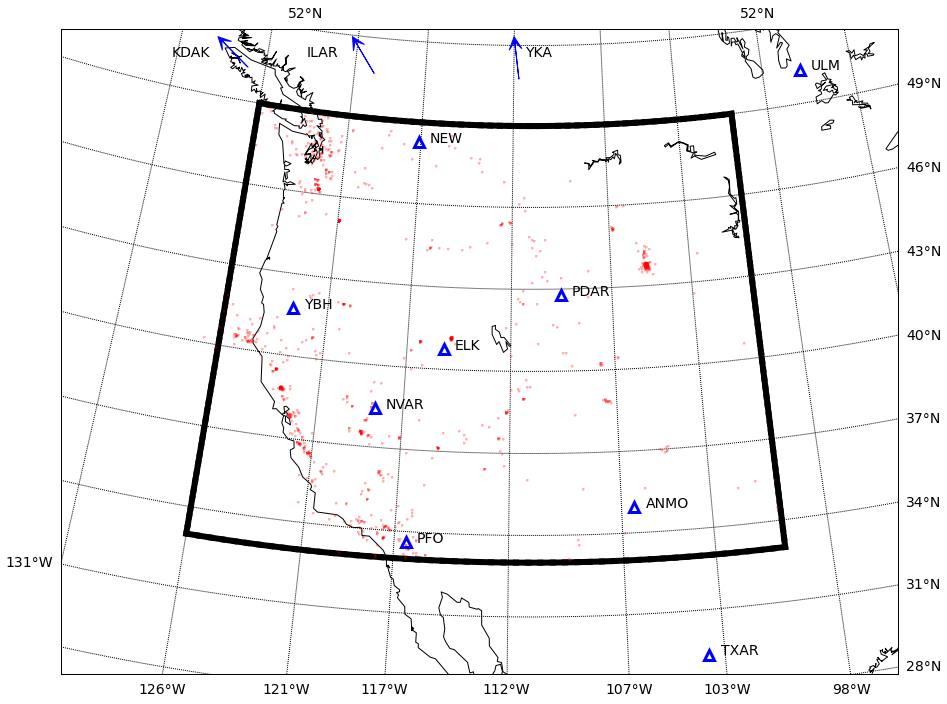
\includegraphics[width=.45\textwidth]{train_stations}
\caption{Training events from the western US dataset, with region of interest outlined
  in black. Triangles indicate IMS stations
  (Table~\ref{tbl:stations}); note that stations KDAK, ILAR, and YKA
  are above the north edge of the map.}
\label{fig:iscevents}
\end{figure}


\begin{figure}
\centering
    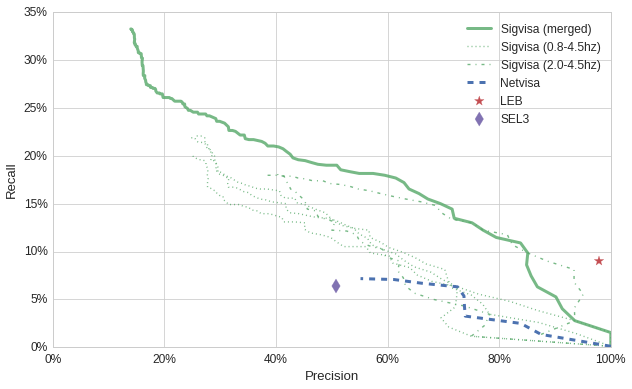
\includegraphics[width=0.45\textwidth]{test_prec_recall}
    \caption{Precision-recall performance over the two-week test
      period, relative to the ISC/UNR reference bulletin.}
  \label{fig:test_prec_recall}
\end{figure}


\begin{figure}
\centering
    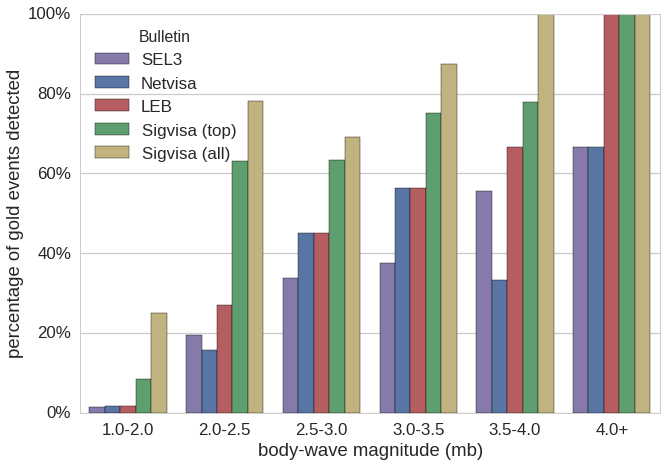
\includegraphics[width=0.45\textwidth]{isc_detections_by_mb}
    \caption{Number of reference events detected, by event
      magnitude. The SIGVISA (top) bulletin is defined to match the
      precision of SEL3 (51\%).}
  \label{fig:isc_evs_by_mb}
\end{figure}


\begin{figure}
\centering
    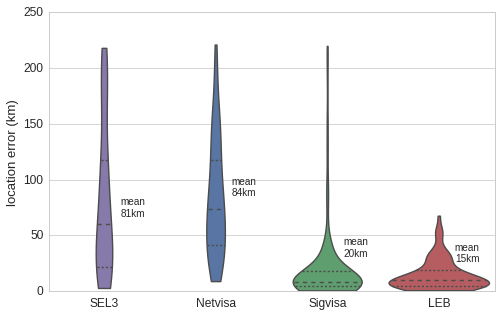
\includegraphics[width=0.45\textwidth]{location_err_violin_test}
    \caption{Distribution of location errors.}
  \label{fig:test_location_err}
\end{figure}


\begin{figure}
\centering
\begin{subfigure}[b]{0.45\textwidth}
%http://kampos.banatao.berkeley.edu:8001/sigvisa/mcmc/d68f03a3-2fb8-412e-852e-59fd7444faf4/waves/wave_PD31_BHZ_freq_0.8_4.5_1204128942.0/vis.png?step=612;stime=1204132610;etime=1204132637.;zoom=2;pred_env=False;pred_signal=True;pred_signal_var=True;plot_predictions=false;clean=true
    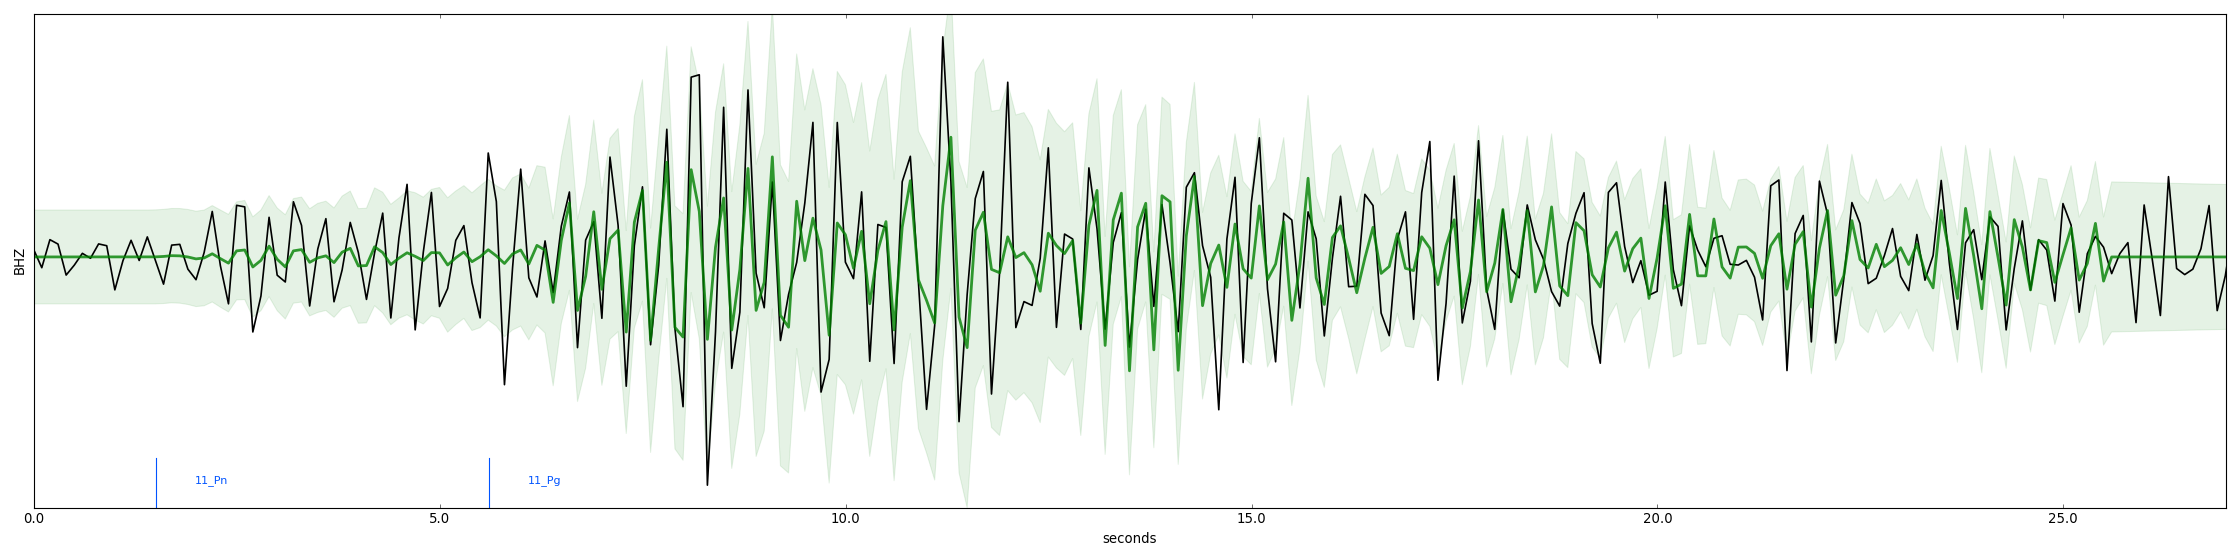
\includegraphics[width=\textwidth]{pd31_missed}
    \caption{Likely mining explosion at Black Thunder Mine. Location 105.21$\deg$ W, 43.75$\deg$ N, depth 1.9km, origin time 17:15:58 UTC, 2008-02-27, mb 2.6, recorded at PDAR (PD31).}
\end{subfigure}

\begin{subfigure}[b]{0.45\textwidth}
%http://kampos.banatao.berkeley.edu:8001/sigvisa/mcmc/5a50e599-15d2-43cc-9a3b-4e0dbe693eba/waves/wave_NV01_sz_freq_0.8_4.5_1204258542.0/vis.png?step=455;stime=1204262510;etime=1204262545;zoom=2;pred_signal=True;pred_signal_var=True;pred_env=False;plot_predictions=false;clean=true
    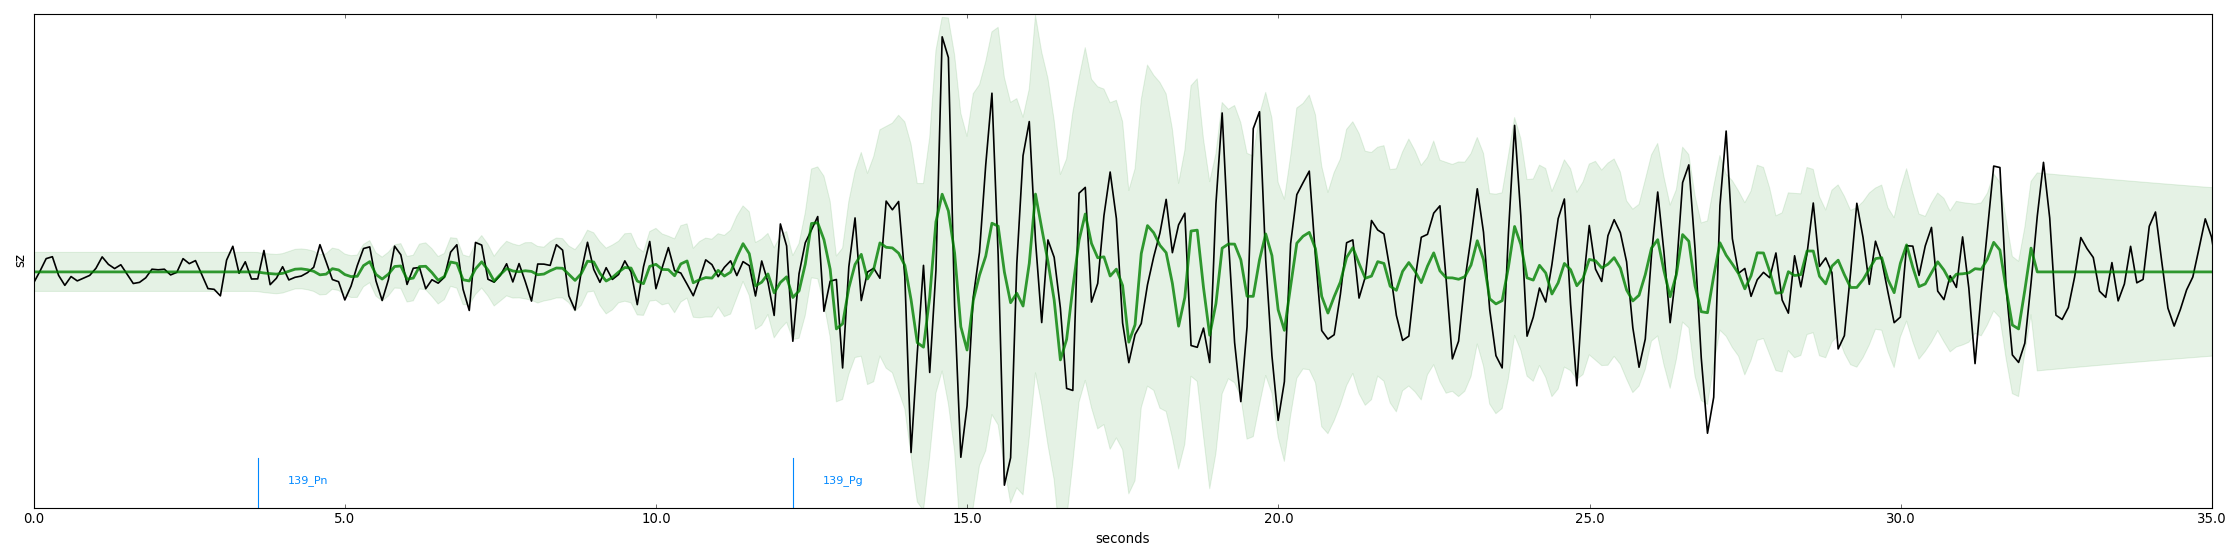
\includegraphics[width=\textwidth]{nv01_missed}
    \caption{Event near Cloverdale, CA along the Rodgers Creek
      fault. Location 122.79$\deg$ W, 38.80$\deg$ N, depth 1.6km,
      origin time 05:20:56 UTC, 2008-02-29,  mb 2.6, recorded at NVAR
      (NV01).}
\end{subfigure}
\caption{Waveform correlation evidence for arriving Pn/Pg phases of two example events detected by SIGVISA
  but not present in the ISC regional bulletin, and thus classified as
  false detections by our evaluation. Green indicates the model
  predicted signal (shaded $\pm 2\sigma$), based on
historical events at each location, while black is the observed
signal (vertical component, filtered 0.8-4.5Hz).}
  \label{fig:sigvisa_genuine_evs}
\end{figure}


\begin{figure*}
\centering
\begin{subfigure}[b]{0.45\textwidth}
\stackinset{r}{}{b}{}{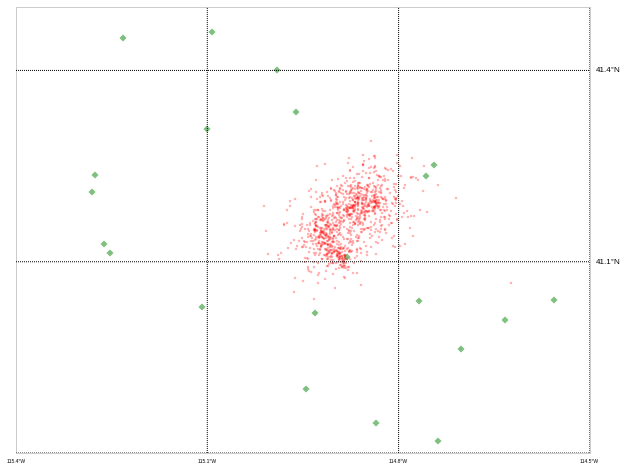
\includegraphics[width=1.2in]{visa_map_wells}}
  {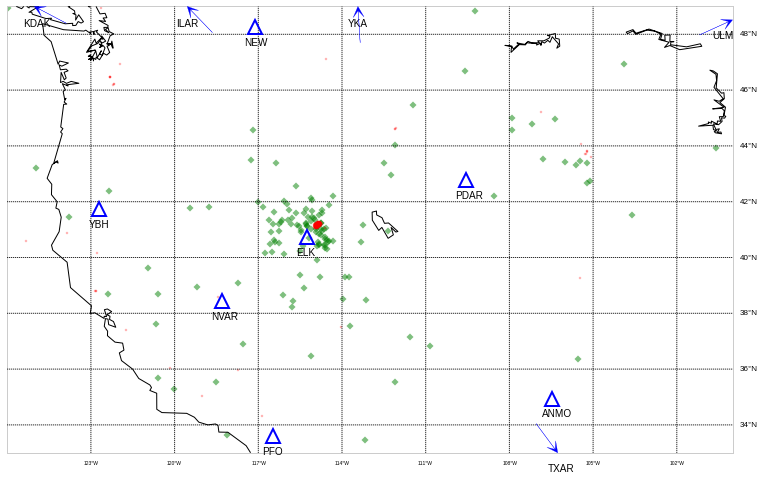
\includegraphics[width=\textwidth]{visa_map}}
\caption{NETVISA (139 events)}
\label{fig:visa_map}
\end{subfigure}
\begin{subfigure}[b]{0.45\textwidth}
\stackinset{r}{}{b}{}{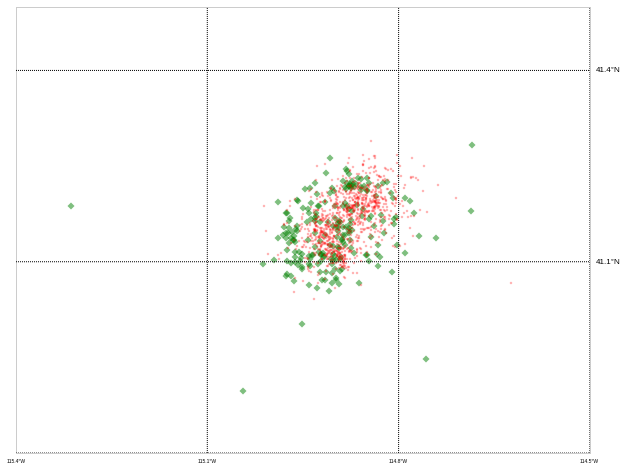
\includegraphics[width=1.2in]{sigvisa_top_map_wells}}
  {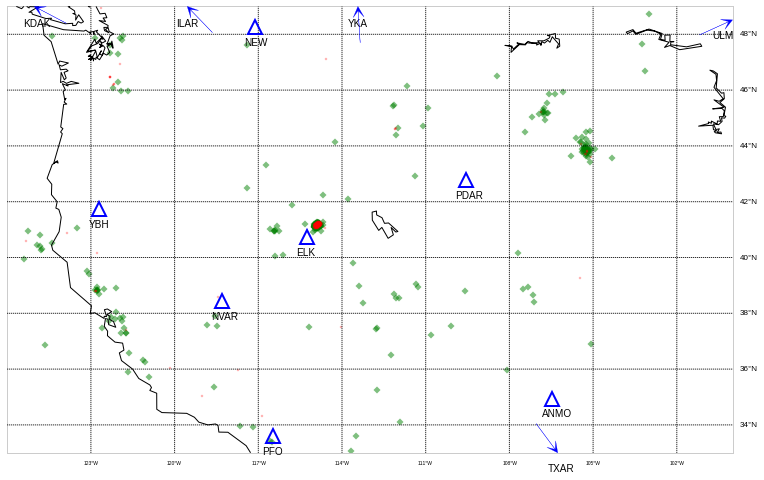
\includegraphics[width=\textwidth]{sigvisa_top_map}}
\caption{SIGVISA top events (393 events)}
\label{fig:sigvisa_map}
\end{subfigure}

\caption{Inferred bulletins, with inset close-up of Wells aftershocks.}
\label{fig:inferred_map}
\end{figure*}



\begin{figure}
\centering

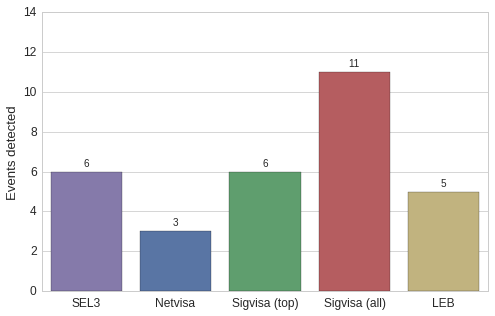
\includegraphics[width=0.45\textwidth]{denovo_recall}
\caption{Recall for 24 {\em de novo} events between January and March
2008. }
\label{fig:denovo_results}
\end{figure}

We consider the task of monitoring seismic events in the western
United States, which contains both significant natural seismicity and
regular mining explosions. We focus in particular on the time period
immediately following the magnitude 6.0 earthquake near Wells, NV, on
February 21, 2008, which generated a large number of aftershocks. We
train on one year of historical data from January 1, 2007, to Dec 31,
2007; the training set also includes the first six hours following the Wells mainshock so
as to enable SIGVISA to recognize aftershocks using waveform correlation. The test period is two weeks long, beginning twelve hours
after the Wells mainshock; the intervening six hours was used as a validation set.

We compare SIGVISA's performance to that of existing monitoring
systems that also process IMS data. SEL3 is the final-stage automated
bulletin from the CTBTO's existing Global Association (GA) system; it
is reviewed by a team of human analysts to produce the Late Event
Bulletin (LEB) reported to the member states. We also compare to
NETVISA \citep{arora2013net}, which implements detection-based
Bayesian monitoring and also generates a fully automated bulletin. All
systems use data from the International Monitoring System; we run
SIGVISA using only the nearest twelve stations to the test region
(\Cref{fig:stations}).

To evaluate the performance of these systems, we construct a reference
bulletin by combining events from regional networks aggregated by the
National Earthquake Information Center (NEIC), the transportable US
Array\footnote{\url{http://www.usarray.org/researchers/obs/transportable}},
and an analysis of aftershocks from the Wells earthquake based on
temporary instruments deployed by the University of Nevada, Reno (UNR)
\citep{smith2011preliminary}; see \todo{long ref} for further
details. Because the reference bulletin has access to many 
sensors not included in the IMS, it is a plausible source of ``ground
truth'' to evaluate the IMS-based systems. 

We trained two sets of SIGVISA models, on
broadband (0.8-4.5Hz) signals as well as a higher-frequency band
(2.0-4.5Hz) intended to provide clearer evidence of regional
events, using events observed from the reference bulletin. 
To produce a test bulletin, we ran three MCMC chains on
broadband signals and two on high-frequency signals, and merged the
results using a greedy heuristic that iteratively selects the
highest-scoring event from any chain excluding duplicates. Each
individual chain was parallelized by dividing the test period into 168
two-hour blocks and running independent inference on each block of
signals. Overall SIGVISA inference used 840 cores for 48 hours.

We evaluate each system by computing a minimum weight maximum
cardinality matching matching between the inferred and reference bulletins, in a bipartite
graph with edges weighted by distance and restricted to
events separated by at most $2\deg$ in distance and 50s in
time. Using this matching, we report precision (the percentage of inferred
events that are real), recall (the percentage of real events detected
by each system), and mean location error of matched events. For
NETVISA and SIGVISA, which attach a confidence score to each event, we
report a precision-recall curve parameterized by the confidence
threshold. 

As shown in \Cref{fig:test_prec_recall}, the merged SIGVISA
bulletin dominates both NETVISA and SEL3. When operating at the same
precision as SEL3 (51\%), SIGVISA achieves recall of 19.3\% versus
SEL3's 6.4\%, also eclipsing the 7.3\% recall achieved by NETVISA at a slightly higher
precision (54.7\%). Unsurprisingly, the analyst-reviewed LEB contains very few
false events, achieving 97.9\% precision relative to our reference
bulletin, at 9.0\% recall. At the other extreme, the full,
un-thresholded SIGVISA bulletin recovers a full 33.3\% of the reference
events, though at the cost of generating many false events (14\% precision). 

Because our analysis is performed with respect to the ISC/UNR
reference bulletin, it may classify as false some genuine events that
occur in regions where this bulletin does not have the same strength
of coverage as for the Wells
aftershocks. \Cref{fig:sigvisa_genuine_evs} shows two such
events inferred by SIGVISA, which are to our eyes likely genuine, due to
strong correspondence between the model-predicted and observed
waveforms, but are not
present in the reference bulletin. The existence of such events provides reason to believe
that SIGVISA's true performance on this dataset is modestly higher than our evaluation
suggests. 


\subsection{de novo events}

For nuclear monitoring it is particularly important
to detect {\em de novo} events: those occurring in locations with no
historical seismicity. We define this as any event whose surface
location is at least $50$km from the
nearest event in the training set. There are only three such events
within the original two-week test period, so we broaden the scope to the
three-month period from January 1, 2008 through March 31, 2008, which
includes twenty-four de novo events. We evaluated each system's recall
specifically of de novo events: of the de novo events in the reference bulletin, how many were detected? 

As shown in \Cref{fig:denovo_results}, SIGVISA's de novo
performance matches or exceeds the other systems. Operating at the
same precision as SEL3, it detects the same number (6/24) of de novo 
events, while achieving comparable location accuracy. Although the
sample size is small, this is encouraging evidence that SIGVISA's
performance on repeated events -- which, to be clear, includes by our
definition almost all of the natural seismicity in the western US during our two-week
test period -- does not come at a cost for de novo events. Indeed,
the full high-sensitivity SIGVISA bulletin includes six events
registered by the ISC but not by any other IMS-based
system. 

\section{Discussion}

Our results demonstrate the promise of 
Bayesian inference on raw waveforms for monitoring seismic
events. Applying MCMC to a generative probability model of repeatable
seismic signals, we recover up to three times as many events as a
detection-based baseline (SEL3) while operating at the same precision,
and reduce mean location errors by a factor of four while greatly increasing
sensitivity to low-magnitude events. Our system maintains effective
performance even for events in regions with no historical seismicity
in the training set.




\subsubsection*{Acknowledgements}


\subsubsection*{References}

\bibliographystyle{apa}
\bibliography{references}

\end{document}
